%
%
%
% ██╗    ██╗ ██████╗ ██╗████████╗███████╗██╗  ██╗
% ██║    ██║██╔═══██╗██║╚══██╔══╝██╔════╝██║ ██╔╝
% ██║ █╗ ██║██║   ██║██║   ██║   █████╗  █████╔╝
% ██║███╗██║██║   ██║██║   ██║   ██╔══╝  ██╔═██╗
% ╚███╔███╔╝╚██████╔╝██║   ██║   ███████╗██║  ██╗
%  ╚══╝╚══╝  ╚═════╝ ╚═╝   ╚═╝   ╚══════╝╚═╝  ╚═╝
%
%
%
% .##.......####...######..######..##..##.
% .##......##..##....##....##.......####..
% .##......######....##....####......##...
% .##......##..##....##....##.......####..
% .######..##..##....##....######..##..##.
%
%
%
\documentclass[8pt,american]{beamer}
\usepackage{amsmath}
\usepackage{amssymb}
\usepackage{babel}
\usepackage{float}
\usepackage[T1]{fontenc}
\usepackage{graphicx}
\usepackage[none]{hyphenat}
\usepackage[utf8]{inputenc}
\usepackage{lmodern}
\usepackage{microtype}
\usepackage{ragged2e}
\setbeamertemplate{footline}{}
\setbeamertemplate{headline}{}
\setbeamertemplate{navigation symbols}{}
\setlength{\parindent}{0pt}
\setlength{\parskip}{\medskipamount}
\usetheme{Rochester}
\usecolortheme{beetle}
\author{Marcio Woitek}
\date{\today}
\title[]{Notes on Neural Networks}

\begin{document}

\frame{\titlepage}

\section[]{Model Representation}

\begin{frame}{Model Representation}

\begin{figure}[H]
\centering
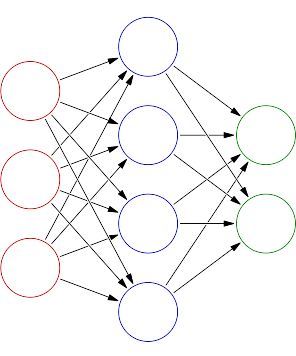
\includegraphics[height=0.8\textheight]{neural_network.png}
\caption{Basic Structure of a Neural Network}
\label{fig:neural_network}
\end{figure}

\end{frame}

\begin{frame}{Model Representation}

\begin{block}{Fundamental Ideas}
\begin{itemize}
\justifying
\item A neural network is formed by nodes or \textit{units}.
\item The units are organized in \textit{layers}.
\item There are at least two layers, the \textit{input layer} and the
  \textit{output layer}.
\item However, very often, between these layers there are
  \textit{hidden layers}.
\item In Fig.~\ref{fig:neural_network}, the red nodes form the input layer, the
  blue nodes form the hidden layer, and the green nodes form the output layer.
\item For simplicity, in the next slides, we discuss the particular case of the
  neural network in this figure.
\end{itemize}
\end{block}

\end{frame}

\begin{frame}{Model Representation}

\begin{block}{Underlying Mathematical Concepts}
\begin{itemize}
\justifying
\item First, consider the input layer.
\item We assume there are $n_{1}$ input units. In the case of
  Fig.~\ref{fig:neural_network}, we have $n_{1}=3$.
\item We denote the input values by $x_{1},x_{2},\ldots,x_{n_{1}}$.
\item There can also be an extra unit, the so-called \textit{bias unit}. Its
  value is represented by $x_{0}$.
\item It is convenient to organize all these values in a single
  $\left(n_{1}+1\right)$-dimensional column vector:
  \begin{equation}
  \mathbf{a}^{\left(1\right)}=\begin{bmatrix}x_{0}\\
  x_{1}\\
  \vdots\\
  x_{n_{1}}
  \end{bmatrix}.
  \end{equation}
\end{itemize}
\end{block}

\end{frame}

\begin{frame}{Model Representation}

\begin{block}{Underlying Mathematical Concepts}
\begin{itemize}
\justifying
\item We can use a similar idea to represent the values related to the other
  layers.
\item To be more precise, we assume the neural network has $L$ layers.
\item Then the values associated with the $j$-th layer will be organized in a
  column vector $\mathbf{a}^{\left(j\right)}$ $\left(j=1,\ldots,L\right)$.
\item The vector $\mathbf{a}^{\left(j\right)}$ is
  $\left(n_{j}+1\right)$-dimensional, where $n_{j}$ denotes the number of units
  in the $j$-th layer.
\item This vector has an extra dimension because the value associated with the
  bias unit of this layer is also included in $\mathbf{a}^{\left(j\right)}$.
\end{itemize}
\end{block}

\end{frame}

\begin{frame}{Model Representation}

\begin{block}{Example of Fig.~\ref{fig:neural_network}}
\begin{itemize}
\justifying
\item As an example, we discuss the neural network in
  Fig.~\ref{fig:neural_network}.
\item Clearly, this network has $L=3$ layers.
\item Then the unit values are organized in 3 vectors,
  $\mathbf{x}=\mathbf{a}^{\left(1\right)}$, $\mathbf{a}^{\left(2\right)}$ and
  $\mathbf{y}=\mathbf{a}^{\left(3\right)}$.
\item From Fig.~\ref{fig:neural_network}, we can see that the numbers of units
  are given by $n_{1}=3$, $n_{2}=4$ and $n_{3}=2$.
\item Therefore, taking into account the values of the bias units, we can state
  the following: $\mathbf{a}^{\left(1\right)}\in\mathbb{R}^{4}$,
  $\mathbf{a}^{\left(2\right)}\in\mathbb{R}^{5}$ and
  $\mathbf{a}^{\left(3\right)}\in\mathbb{R}^{3}$.
\end{itemize}
\end{block}

\end{frame}

\section[]{Forward Propagation}

\begin{frame}{Forward Propagation}

\begin{block}{}
\begin{itemize}
\justifying
\item Next, we explain how the input values are propagated in the network.
\item Essentially, we start from the input vector
  $\mathbf{x}=\mathbf{a}^{\left(1\right)}$, and map
  $\mathbf{a}^{\left(j\right)}$ to $\mathbf{a}^{\left(j+1\right)}$ until we
  obtain the output vector $\mathbf{y}=\mathbf{a}^{\left(L\right)}$.
\item In our example, the idea is the following: first, the input vector
  $\mathbf{x}=\mathbf{a}^{\left(1\right)}$ is mapped to
  $\mathbf{a}^{\left(2\right)}$, and then this vector is mapped to
  $\mathbf{a}^{\left(3\right)}$, producing the output $\mathbf{y}$.
\item To be specific about how these mappings work, we introduce 2 vectors,
  $\mathbf{z}^{\left(2\right)}$ and $\mathbf{z}^{\left(3\right)}$.
\item In general, we introduce $L-1$ vectors $\mathbf{z}^{\left(j\right)}$,
  where $j=2,\ldots,L$.
\item We also define a set with $L-1$ functions $g^{\left(j\right)}$, where
  $j=2,\ldots,L$. The function $g^{\left(j\right)}$ is called the
  \textit{activation function} of the $j$-th layer. Notice that there isn't an
  activation function associated with the input layer.
\item To discuss our example, we consider the particular case in which all
  activation functions are the same. We denote this function by $h$.
\end{itemize}
\end{block}

\end{frame}

\begin{frame}{Forward Propagation}

\begin{block}{Activation Function}
\begin{itemize}
\justifying
\item For the activation functions, there are many choices.
\item To discuss our example, we consider the particular case in which $h$ is
  the \textit{sigmoid} or \textit{logistic function}:
  \begin{equation}
  h\left(x\right)=\frac{1}{1+\exp\left(-x\right)}.
  \label{eq:defn_sigm}
  \end{equation}
\end{itemize}
\begin{figure}[H]
\centering
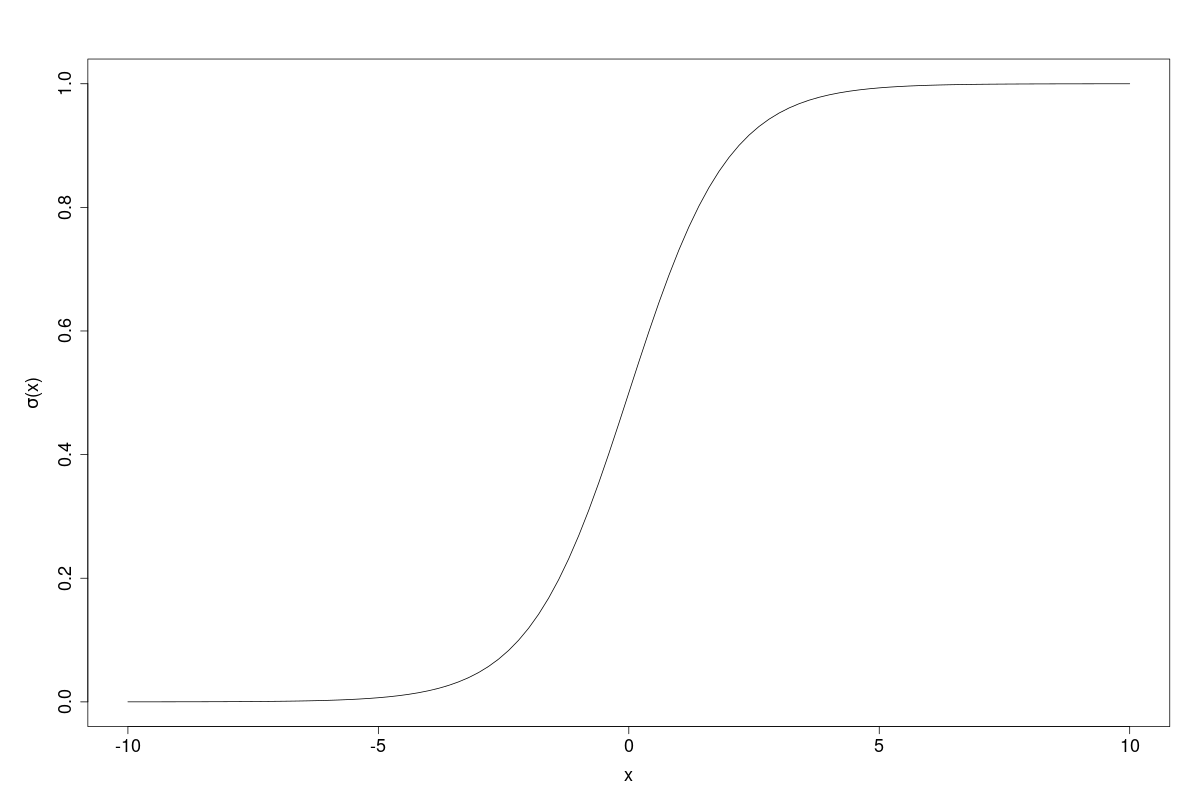
\includegraphics[height=0.4\textheight]{../r/sigmoid.png}
\caption{Graph of the sigmoid function.}
\label{fig:graph_sigm}
\end{figure}
\end{block}

\end{frame}

\begin{frame}{Forward Propagation}

\begin{block}{Forward Propagation Equations}
\begin{itemize}
\justifying
\item We continue by explaining how the vector $\mathbf{z}^{\left(j\right)}$ is
  computed from the unit values in $\mathbf{a}^{\left(j-1\right)}$.
\item We imagine all units in the $\left(j-1\right)$-th layer (including the
  bias unit) are connected to every unit in the $j$-th layer (excluding the
  bias unit).
\item Then between these layers there are $\left(n_{j-1}+1\right)n_{j}$
  connections.
\item Each of these connections has a different \textit{weight}. We will
  organize all these weights in a matrix denoted by $\Theta^{\left(j-1\right)}$.
\item The element $\Theta_{ik}^{\left(j-1\right)}$ in the $i$-th row and $k$-th
  column of this matrix is interpreted as follows: it is the weight of the
  connection between the $k$-th unit in the $\left(j-1\right)$-th layer and the
  $i$-th unit in the $j$-th layer.
\item Then the dimension of the matrix $\Theta^{\left(j-1\right)}$ is
  $n_{j}\times\left(n_{j-1}+1\right)$.
\end{itemize}
\end{block}

\end{frame}

\begin{frame}{Forward Propagation}

\begin{block}{Forward Propagation Equations}
\begin{itemize}
\justifying
\item Finally, we can write down the equations that determine the vector
  $\mathbf{z}^{\left(j\right)}$.
\item The $i$-th component of this vector is given by the \textit{weighted sum}
  of the components of $\mathbf{a}^{\left(j-1\right)}$:
  \begin{align}
  \nonumber z_{i}^{\left(j\right)}&=\Theta_{i0}^{\left(j-1\right)}a_{0}^{\left(j-1\right)}+\Theta_{i1}^{\left(j-1\right)}a_{1}^{\left(j-1\right)}+\ldots+\Theta_{i,n_{j-1}}^{\left(j-1\right)}a_{n_{j-1}}^{\left(j-1\right)}\\
  &=\sum_{k=0}^{n_{j-1}}\Theta_{ik}^{\left(j-1\right)}a_{k}^{\left(j-1\right)}.
  \end{align}
\item The last expression can be written in matrix form as follows:
  \begin{equation}
  \mathbf{z}^{\left(j\right)}=\Theta^{\left(j-1\right)}\mathbf{a}^{\left(j-1\right)}.
  \end{equation}
\end{itemize}
\end{block}

\end{frame}

\begin{frame}{Forward Propagation}

\begin{block}{Forward Propagation Equations}
\begin{itemize}
\justifying
\item Now, to obtain the vector $\mathbf{a}^{\left(j\right)}$, we only need to
  apply the activation function $g^{\left(j\right)}$ to every component of
  $\mathbf{z}^{\left(j\right)}$:
  \begin{equation}
  \mathbf{a}^{\left(j\right)}=g^{\left(j\right)}\left(\mathbf{z}^{\left(j\right)}\right)=\begin{bmatrix}g^{\left(j\right)}\left(z_{1}^{\left(j\right)}\right)\\
  g^{\left(j\right)}\left(z_{2}^{\left(j\right)}\right)\\
  \vdots\\
  g^{\left(j\right)}\left(z_{n_{j}}^{\left(j\right)}\right)
  \end{bmatrix}.
  \end{equation}
\item .
\end{itemize}
\end{block}

\end{frame}

\end{document}
